% Do information-theoretic causality measures agree?
% Lecture slides for students new to information theory and causal inference.
%
% Build:  uv run experiments/slide_figures.py   (regenerates figures/ from results/)
%         tectonic slides.tex                    (or: latexmk -xelatex slides.tex)

\documentclass[aspectratio=169,11pt,xcolor={table}]{beamer}

\usepackage{amsmath,amssymb}
\usepackage{booktabs}
\usepackage{pifont}
\usepackage{tikz}
\usetikzlibrary{arrows.meta,positioning,calc,decorations.pathreplacing}
\graphicspath{{figures/}}

% ---------------------------------------------------------------- colors
\definecolor{ink}{HTML}{0B0B0B}
\definecolor{muted}{HTML}{52514E}
\definecolor{accent}{HTML}{1C5CAB}
\definecolor{surface}{HTML}{FCFCFB}
\definecolor{panel}{HTML}{F0EFEC}
\definecolor{sBlue}{HTML}{2A78D6}
\definecolor{sOrange}{HTML}{EB6834}
\definecolor{sAqua}{HTML}{1BAF7A}
\definecolor{sYellow}{HTML}{EDA100}
\definecolor{sGray}{HTML}{9A9993}
\definecolor{flag}{HTML}{FBE1D6}

% ---------------------------------------------------------------- theme
\setbeamercolor{background canvas}{bg=surface}
\setbeamercolor{normal text}{fg=ink}
\setbeamercolor{structure}{fg=accent}
\setbeamercolor{frametitle}{fg=ink}
\setbeamercolor{title}{fg=ink}
\setbeamercolor{subtitle}{fg=muted}
\setbeamercolor{block title}{fg=ink,bg=panel}
\setbeamercolor{block body}{fg=ink,bg=panel!45}
\setbeamerfont{frametitle}{series=\bfseries,size=\large}
\setbeamerfont{title}{series=\bfseries,size=\LARGE}
\setbeamerfont{block title}{series=\bfseries,size=\small}
\setbeamertemplate{navigation symbols}{}
\setbeamertemplate{itemize items}[circle]
\setbeamertemplate{enumerate items}[default]
\setbeamertemplate{blocks}[rounded]
\setbeamertemplate{footline}{%
  \hspace*{4mm}{\color{muted}\scriptsize\insertsection}\hfill
  {\color{muted}\scriptsize\insertframenumber}\hspace*{4mm}\vspace*{3mm}}

\AtBeginSection{%
  \begin{frame}[plain,noframenumbering]{Where we are}
    \tableofcontents[currentsection,hideallsubsections]
  \end{frame}}

% ---------------------------------------------------------------- notation
\newcommand{\Xt}{X_t}
\newcommand{\Yt}{Y_t}
\newcommand{\Yn}{Y_{t+1}}
\newcommand{\bits}{\text{ bits}}
\newcommand{\cmark}{{\color{sAqua}\ding{51}}}
\newcommand{\xmark}{{\color{sOrange}\ding{55}}}
\newcommand{\flagged}[1]{\cellcolor{flag}#1}
\newcommand{\aside}[1]{{\color{muted}\small #1}}

% ---------------------------------------------------------------- tikz styles
\tikzset{
  var/.style={circle, draw=ink, line width=0.7pt, minimum size=9.5mm, inner sep=0pt,
              font=\small, fill=white},
  key/.style={var, fill=accent!13},
  hid/.style={var, dashed, draw=muted, fill=panel, text=muted},
  known/.style={var, fill=panel},
  setvar/.style={rectangle, rounded corners=2pt, draw=ink, line width=0.9pt, minimum size=8.5mm,
                 inner sep=1pt, font=\small, fill=accent!13},
  arr/.style={-{Stealth[length=2.3mm,width=1.9mm]}, line width=0.8pt, draw=ink},
  gone/.style={arr, draw=sGray, dashed},
  noarrow/.style={-{Stealth[length=2.3mm,width=1.9mm]}, line width=0.8pt, draw=sOrange, dashed},
  word/.style={rectangle, rounded corners=7pt, draw=ink, line width=0.7pt, minimum height=8mm,
               minimum width=15mm, inner sep=3pt, font=\footnotesize, align=center, fill=white},
  lab/.style={font=\scriptsize, text=muted},
  tick/.style={font=\scriptsize, text=muted},
}

% ---------------------------------------------------------------- title
\title{Do information-theoretic\\causality measures agree?}
\subtitle{Transfer entropy, information flow and causal strength\\on tiny systems we can solve exactly}
\author{Michael Rowlands}
\date{}

\begin{document}

\begin{frame}[plain,noframenumbering]
  \titlepage
\end{frame}

% ====================================================================
\begin{frame}{A puzzle}
  Two binary signals, recorded once per time step (filled = 1):
  \begin{center}
  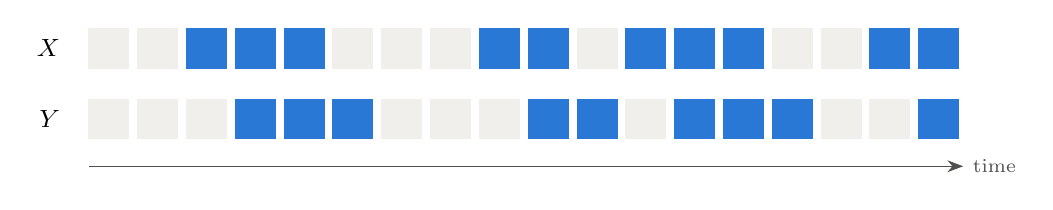
\begin{tikzpicture}[x=6.2mm]
    \node[anchor=east, font=\small] at (0.2,0) {$X$};
    \node[anchor=east, font=\small] at (0.2,-0.9) {$Y$};
    \foreach \v [count=\i] in {0,0,1,1,1,0,0,0,1,1,0,1,1,1,0,0,1,1} {
      \ifnum\v=1 \fill[sBlue] (\i-0.42,-0.26) rectangle (\i+0.42,0.26);
      \else \fill[panel] (\i-0.42,-0.26) rectangle (\i+0.42,0.26); \fi }
    \foreach \v [count=\i] in {0,0,0,1,1,1,0,0,0,1,1,0,1,1,1,0,0,1} {
      \ifnum\v=1 \fill[sBlue] (\i-0.42,-1.16) rectangle (\i+0.42,-0.64);
      \else \fill[panel] (\i-0.42,-1.16) rectangle (\i+0.42,-0.64); \fi }
    \draw[-{Stealth[length=2mm]}, muted] (0.6,-1.5) -- (18.5,-1.5) node[right, lab] {time};
  \end{tikzpicture}
  \end{center}
  \vspace{-2mm}
  $Y$ looks exactly like $X$, one step later. So\ldots
  \begin{itemize}
    \item Does $X$ \emph{drive} $Y$?
    \item Or does some third thing drive both, reaching $X$ first?
    \item And how would we put a \emph{number} on ``how much $X$ influences $Y$''?
  \end{itemize}
  \medskip
  Scientists ask this about brain regions, climate indices and stock prices.
  A popular tool is \textbf{transfer entropy}, often described as ``information flowing from $X$ to $Y$''.
  Today: when does that description hold, and when does it fail?
\end{frame}

\begin{frame}{The plan}
  \begin{columns}[T]
    \begin{column}{0.48\textwidth}
      \textbf{Three measures} of ``how much $X$ influences $Y$''
      \begin{enumerate}
        \item Transfer entropy \aside{(Schreiber, 2000)}
        \item Information flow \aside{(Ay \& Polani, 2008)}
        \item Causal strength \aside{(Janzing et al., 2013)}
      \end{enumerate}
      \medskip
      \textbf{Three toy systems} built so they disagree
      \begin{enumerate}
        \item a hidden common driver
        \item an XOR (``it takes two'')
        \item a slowly changing signal that is copied
      \end{enumerate}
    \end{column}
    \begin{column}{0.48\textwidth}
      \begin{block}{Why toy systems?}
        Every variable is a single bit, so each system has at most $2^5 = 32$ possible outcomes.
        We can write down the \emph{whole} probability table and compute every measure
        \textbf{exactly}.\\[1mm]
        No data, no sampling noise: if two measures disagree, the disagreement is
        about what they \emph{mean}, not about statistics.
      \end{block}
      \smallskip
      \aside{First we need two toolkits: measuring information in bits, and talking precisely about causes.}
    \end{column}
  \end{columns}
\end{frame}

% ====================================================================
\section{Information in bits}

\begin{frame}{Entropy: uncertainty measured in bits}
  \begin{columns}[c]
    \begin{column}{0.53\textwidth}
      For a random variable $X$ with probabilities $p(x)$:
      \[ H(X) = -\sum_x p(x)\,\log_2 p(x) \]
      \begin{itemize}
        \item The average number of yes/no questions needed to guess $X$.
        \item Fair coin: $H = 1$ bit.
        \item Coin with $P(\text{heads}) = 0.9$: $H \approx 0.47$ bits. It is easier to guess.
        \item A coin that always lands heads: $H = 0$.
      \end{itemize}
      \smallskip
      For a biased coin we write $h(p)$, the \emph{binary entropy}.
    \end{column}
    \begin{column}{0.44\textwidth}
      \centering
      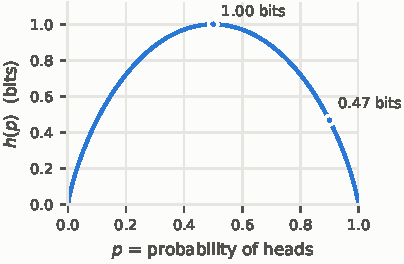
\includegraphics[width=\linewidth]{binary_entropy.pdf}
    \end{column}
  \end{columns}
\end{frame}

\begin{frame}{Mutual information: what one variable tells you about another}
  \begin{columns}[c]
    \begin{column}{0.52\textwidth}
      \[ I(X;Y) = H(Y) - H(Y \mid X) \]
      The bits of uncertainty about $Y$ that knowing $X$ removes.
      \begin{itemize}
        \item Symmetric: $I(X;Y) = I(Y;X)$.
        \item $I(X;Y) = 0$ exactly when $X$ and $Y$ are independent.
      \end{itemize}
      \medskip
      \textbf{Examples} with a fair coin $X$:
      \begin{itemize}
        \item $Y = X$: \quad $I = 1$ bit
        \item $Y$ an unrelated coin: \quad $I = 0$
        \item $Y = X$, but flipped with probability $\varepsilon$: \quad $I = 1 - h(\varepsilon)$
      \end{itemize}
    \end{column}
    \begin{column}{0.45\textwidth}
      \centering
      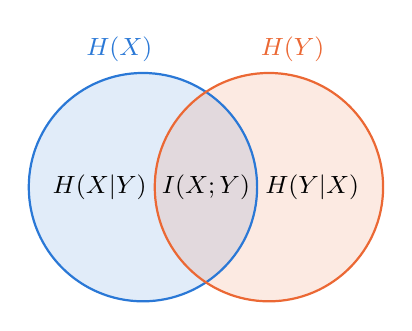
\begin{tikzpicture}
        \fill[sBlue, opacity=0.14] (0,0) circle (1.45);
        \fill[sOrange, opacity=0.14] (1.6,0) circle (1.45);
        \draw[sBlue, line width=0.8pt] (0,0) circle (1.45);
        \draw[sOrange, line width=0.8pt] (1.6,0) circle (1.45);
        \node[font=\small] at (-0.55,0) {$H(X|Y)$};
        \node[font=\small] at (2.15,0) {$H(Y|X)$};
        \node[font=\small] at (0.8,0) {$I(X;Y)$};
        \node[font=\small, text=sBlue] at (-0.3,1.75) {$H(X)$};
        \node[font=\small, text=sOrange] at (1.9,1.75) {$H(Y)$};
      \end{tikzpicture}\\[1mm]
      \aside{The overlap is the information $X$ and $Y$ share.}
    \end{column}
  \end{columns}
\end{frame}

\begin{frame}{Conditional mutual information: what's new, given what you know}
  \vspace{-2mm}
  \[ I(X;Y \mid Z) = H(Y \mid Z) - H(Y \mid X, Z) \]
  What $X$ tells you about $Y$ \emph{once you already know $Z$}. Conditioning can move it either way:
  \smallskip
  \begin{columns}[T]
    \begin{column}{0.47\textwidth}
      \begin{block}{It can remove dependence}
        \centering
        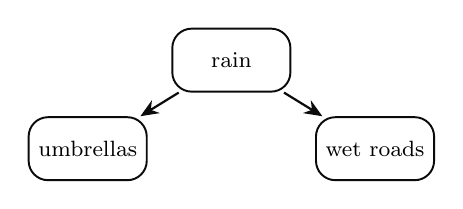
\begin{tikzpicture}[node distance=3mm and 3mm]
          \node[word] (z) {rain};
          \node[word, below left=of z] (x) {umbrellas};
          \node[word, below right=of z] (y) {wet roads};
          \draw[arr] (z) -- (x); \draw[arr] (z) -- (y);
        \end{tikzpicture}\par\smallskip
        \raggedright\small
        Umbrellas predict wet roads: $I(X;Y) > 0$.
        Once you know whether it rained, umbrellas add nothing: $I(X;Y \mid Z) = 0$.
      \end{block}
    \end{column}
    \begin{column}{0.47\textwidth}
      \begin{block}{It can create dependence}
        \centering\small
        $Y = X \oplus Z$, the XOR of two fair coins:\par\smallskip
        \begin{tabular}{@{}ccc@{\hspace{7mm}}ccc@{}}
          \toprule $X$ & $Z$ & $Y$ & $X$ & $Z$ & $Y$ \\ \midrule
          0 & 0 & 0 & 1 & 0 & 1 \\ 0 & 1 & 1 & 1 & 1 & 0 \\ \bottomrule
        \end{tabular}\par\smallskip
        \raggedright
        Alone, $X$ says nothing about $Y$: $I(X;Y) = 0$.
        Given $Z$, $X$ decides $Y$: $I(X;Y \mid Z) = 1$ bit.
      \end{block}
    \end{column}
  \end{columns}
\end{frame}

\begin{frame}{Relative entropy: how different are two distributions?}
  \begin{columns}[c]
    \begin{column}{0.56\textwidth}
      \[ D(P \,\|\, Q) = \sum_x P(x)\, \log_2 \frac{P(x)}{Q(x)} \]
      Also called the \emph{Kullback--Leibler divergence}.
      \begin{itemize}
        \item The extra bits you pay, on average, if the world follows $P$ but you planned for $Q$.
        \item Always $\ge 0$, and $= 0$ exactly when $P = Q$.
        \item Not symmetric, so not a true distance.
      \end{itemize}
      \medskip
      Example: $P$ = fair coin, $Q$ = 90/10 coin gives $D(P\|Q) \approx 0.74$ bits.
    \end{column}
    \begin{column}{0.4\textwidth}
      \begin{block}{Mutual information is a relative entropy}
        \[ I(X;Y) = D\big(P(x,y) \,\|\, P(x)\,P(y)\big) \]
        How far the real joint distribution is from ``$X$ and $Y$ independent''.
      \end{block}
      \smallskip
      \aside{We'll use this idea again: one causal measure compares the real world with a world where a link is cut.}
    \end{column}
  \end{columns}
\end{frame}

% ====================================================================
\section{Causes and interventions}

\begin{frame}{Correlation is not causation}
  \begin{columns}[c]
    \begin{column}{0.5\textwidth}
      Ice cream sales and swimming accidents rise and fall together.
      Does ice cream cause accidents?\\[2mm]
      No: hot weather drives both. It is a \textbf{common cause}, or \textbf{confounder}.
      \bigskip

      A \textbf{causal graph} draws this:
      \begin{itemize}
        \item one node per variable,
        \item an arrow $A \to B$ when $A$ is a \emph{direct input} to the mechanism that produces $B$.
      \end{itemize}
    \end{column}
    \begin{column}{0.45\textwidth}
      \centering
      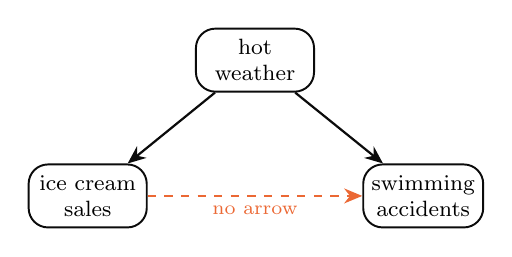
\begin{tikzpicture}[node distance=9mm and 6mm]
        \node[word] (z) {hot\\weather};
        \node[word, below left=of z] (x) {ice cream\\sales};
        \node[word, below right=of z] (y) {swimming\\accidents};
        \draw[arr] (z) -- (x);
        \draw[arr] (z) -- (y);
        \draw[noarrow] (x) -- node[below, font=\scriptsize, text=sOrange] {no arrow} (y);
      \end{tikzpicture}\\[2mm]
      \aside{Ice cream \emph{predicts} accidents,\\but doesn't \emph{cause} them.}
    \end{column}
  \end{columns}
\end{frame}

\begin{frame}{Seeing versus doing}
  \begin{columns}[T]
    \begin{column}{0.46\textwidth}
      \textbf{Seeing}: $P(Y \mid X = x)$\\
      Among the days when $X$ \emph{happened} to be $x$, how is $Y$ distributed?
      \medskip

      \textbf{Doing}: $P(Y \mid \mathrm{do}(X = x))$\\
      Reach in and \emph{force} $X = x$, as in an experiment, overriding whatever normally sets $X$.
      \medskip

      In the graph, forcing $X$ means \textbf{deleting the arrows into $X$}.
    \end{column}
    \begin{column}{0.5\textwidth}
      \centering
      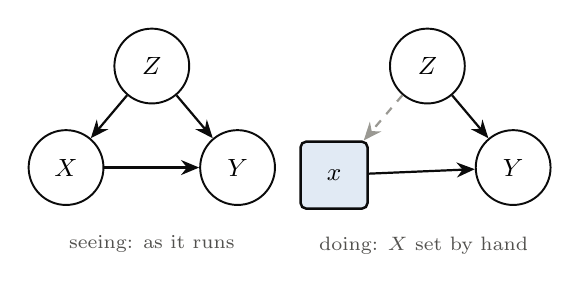
\begin{tikzpicture}[node distance=6mm and 4mm]
        \node[var] (z) {$Z$};
        \node[var, below left=of z] (x) {$X$};
        \node[var, below right=of z] (y) {$Y$};
        \draw[arr] (z) -- (x); \draw[arr] (z) -- (y); \draw[arr] (x) -- (y);
        \node[lab, below=2.5mm of $(x.south)!0.5!(y.south)$] {seeing: as it runs};
        \begin{scope}[xshift=3.5cm]
          \node[var] (z2) {$Z$};
          \node[setvar, below left=of z2] (x2) {$x$};
          \node[var, below right=of z2] (y2) {$Y$};
          \draw[gone] (z2) -- (x2); \draw[arr] (z2) -- (y2); \draw[arr] (x2) -- (y2);
          \node[lab, below=2.5mm of $(x2.south)!0.5!(y2.south)$] {doing: $X$ set by hand};
        \end{scope}
      \end{tikzpicture}
      \par\medskip
      \begin{block}{Ice cream again}
        \small There is no arrow from ice cream to accidents, so handing out free ice cream changes nothing:
        $P(\text{acc.} \mid \mathrm{do}(\text{ice cream})) = P(\text{acc.})$.
        Seeing mixes in whatever travels with $X$; doing isolates $X$ itself.
      \end{block}
    \end{column}
  \end{columns}
\end{frame}

\begin{frame}{Computing $\mathrm{do}(\cdot)$ when you know the graph}
  A causal model is a graph plus one \textbf{mechanism} per variable, $P(v \mid \text{parents of } v)$:
  \[ P(v_1, \dots, v_n) = \prod_i P(v_i \mid \mathrm{pa}_i) \]
  To compute $\mathrm{do}(X = x)$, delete $X$'s mechanism, set $X = x$, and keep every other mechanism:
  \[ P(v \mid \mathrm{do}(X = x)) = \prod_{i \ne X} P(v_i \mid \mathrm{pa}_i) \Big|_{X = x} \]
  \vspace{-2mm}
  \begin{columns}[T]
    \begin{column}{0.55\textwidth}
      For the graph on the previous slide:
      \begin{align*}
        P(y \mid \mathrm{do}(x)) &= \textstyle\sum_z P(z)\, P(y \mid x, z)\\
        P(y \mid x)              &= \textstyle\sum_z P(z \mid x)\, P(y \mid x, z)
      \end{align*}
      They differ exactly when $Z$ travels with $X$.
    \end{column}
    \begin{column}{0.41\textwidth}
      \begin{block}{The catch}
        \small You need the \emph{graph}. The same data can fit several graphs,
        and data alone can't always tell you which way the arrows point.
      \end{block}
    \end{column}
  \end{columns}
\end{frame}

\begin{frame}{Time series as causal graphs}
  \begin{columns}[c]
    \begin{column}{0.5\textwidth}
      Unroll time: every variable at every step gets its own node.
      Causes come before their effects.
      \bigskip

      \textbf{The question for the rest of the talk:}
      \begin{center}
        How much does $\Xt$ influence $\Yn$?
      \end{center}
      \medskip
      $\Yt$ is the target's \emph{own past}. Keep an eye on it.
      \bigskip

      \aside{All variables are bits, and each process has been running long enough to be
      stationary: its statistics don't change over time.}
    \end{column}
    \begin{column}{0.46\textwidth}
      \centering
      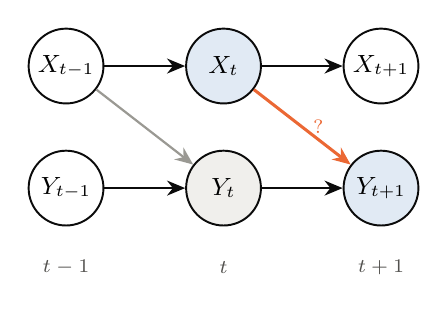
\begin{tikzpicture}[x=2cm, y=1.55cm]
        \node[var] (x0) at (0,0) {$X_{t-1}$};
        \node[key] (x1) at (1,0) {$X_t$};
        \node[var] (x2) at (2,0) {$X_{t+1}$};
        \node[var] (y0) at (0,-1) {$Y_{t-1}$};
        \node[known] (y1) at (1,-1) {$Y_t$};
        \node[key] (y2) at (2,-1) {$Y_{t+1}$};
        \draw[arr] (x0) -- (x1); \draw[arr] (x1) -- (x2);
        \draw[arr] (y0) -- (y1); \draw[arr] (y1) -- (y2);
        \draw[arr, draw=sOrange, line width=1.1pt] (x1) -- node[right, font=\scriptsize, text=sOrange] {?} (y2);
        \draw[arr, draw=sGray] (x0) -- (y1);
        \foreach \t/\l in {0/t-1, 1/t, 2/t+1} \node[tick] at (\t,-1.65) {$\l$};
      \end{tikzpicture}
    \end{column}
  \end{columns}
\end{frame}

% ====================================================================
\section{Three measures of influence}

\begin{frame}{Measure 1: transfer entropy}
  \begin{columns}[c]
    \begin{column}{0.58\textwidth}
      \[ \mathrm{TE}(X \to Y) = I(\Yn;\, \Xt \mid \Yt) \]
      ``Does $X$'s present help predict $Y$'s next value,
      \emph{beyond} what $Y$'s own past already tells us?''
      \medskip
      \[ = H(\Yn \mid \Yt) - H(\Yn \mid \Yt, \Xt) \]
      \vspace{-3mm}
      \begin{itemize}
        \item[\cmark] Needs only observed data: no graph, no experiments.
        \item[\cmark] Widely used, and often read as ``information flow from $X$ to $Y$''.
        \item[\xmark] Purely \emph{predictive}. It never asks what would happen under an intervention.
      \end{itemize}
    \end{column}
    \begin{column}{0.38\textwidth}
      \centering
      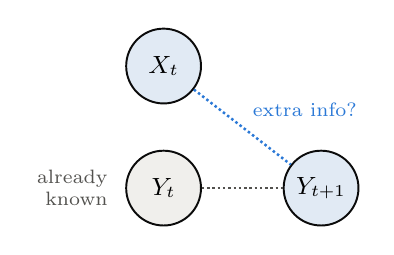
\begin{tikzpicture}[x=2cm, y=1.55cm]
        \node[key] (x1) at (0,0) {$X_t$};
        \node[known] (y1) at (0,-1) {$Y_t$};
        \node[key] (y2) at (1,-1) {$Y_{t+1}$};
        \draw[densely dotted, line width=0.9pt, sBlue] (x1) -- node[above right, font=\scriptsize] {extra info?} (y2);
        \draw[densely dotted, line width=0.9pt, muted] (y1) -- (y2);
        \node[lab, left=1mm of y1, align=right] {already\\known};
      \end{tikzpicture}\\[3mm]
      \aside{Schreiber, \emph{Phys.\ Rev.\ Lett.} 2000.}
    \end{column}
  \end{columns}
\end{frame}

\begin{frame}{Measure 2: information flow (Ay \& Polani)}
  \begin{columns}[c]
    \begin{column}{0.58\textwidth}
      A thought experiment: \textbf{set $X_t$ by hand}, at random with its usual frequencies,
      and watch $\Yn$.
      \smallskip

      $I(\Xt \to \Yn)$ is the mutual information between the value you set and $\Yn$.
      \medskip

      \textbf{Imposing a set $S$} (the hat means ``set by hand''): also fix $S$ by intervention,
      then ask how much $\Xt$ still matters. This gives $I(\Xt \to \Yn \mid \hat S)$.
      We impose $S = \{\Yt\}$, plus any other input to $\Yn$.
    \end{column}
    \begin{column}{0.38\textwidth}
      \centering
      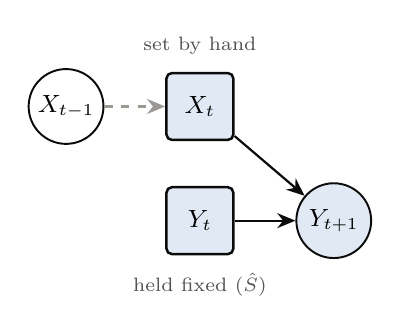
\begin{tikzpicture}[x=1.7cm, y=1.45cm]
        \node[var] (x0) at (0,0) {$X_{t-1}$};
        \node[setvar] (x1) at (1,0) {$X_t$};
        \node[setvar] (y1) at (1,-1) {$Y_t$};
        \node[key] (y2) at (2,-1) {$Y_{t+1}$};
        \draw[gone] (x0) -- (x1);
        \draw[arr] (x1) -- (y2); \draw[arr] (y1) -- (y2);
        \node[lab, above=1mm of x1] {set by hand};
        \node[lab, below=1mm of y1] {held fixed ($\hat S$)};
      \end{tikzpicture}
    \end{column}
  \end{columns}
  \medskip
  \begin{columns}[T]
    \begin{column}{0.5\textwidth}
      \begin{itemize}
        \item[\cmark] Genuinely causal: it measures the response to interventions.
        \item[\xmark] Needs the causal graph, to compute $\mathrm{do}(\cdot)$.
      \end{itemize}
      \aside{Ay \& Polani, \emph{Adv.\ Complex Syst.} 2008.}
    \end{column}
    \begin{column}{0.46\textwidth}
      \begin{block}{Formally}
        \small
        $\hat p(s,x,y) = p(s)\; p(x \mid \mathrm{do}(s))\; p(y \mid \mathrm{do}(s, x))$\\[1mm]
        flow $= I_{\hat p}(X; Y \mid S)$, an ordinary conditional MI.
      \end{block}
    \end{column}
  \end{columns}
\end{frame}

\begin{frame}{Measure 3: causal strength (Janzing et al.)}
  \begin{columns}[c]
    \begin{column}{0.56\textwidth}
      Think of the arrow $\Xt \to \Yn$ as a \textbf{wire}. \textbf{Cut it}, and feed $Y$'s input
      with an independent random copy $X'_t$ that has the same statistics as $\Xt$.
      \[ C_{X \to Y} = D\big(P \,\|\, P_{\text{cut}}\big) \]
      The relative entropy between the real world and the world with the wire cut.
      \begin{itemize}
        \item $C = 0$ exactly when cutting changes nothing, e.g.\ when there is no wire.
        \item For a lone arrow $X \to Y$, $C = I(X;Y)$.
        \item[\xmark] Also needs the causal graph.
      \end{itemize}
    \end{column}
    \begin{column}{0.4\textwidth}
      \centering
      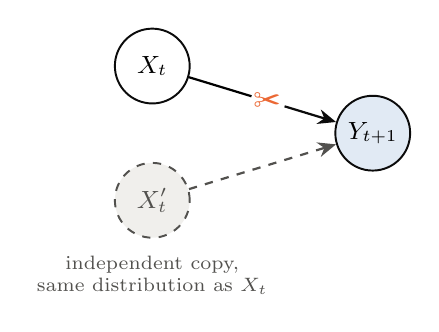
\begin{tikzpicture}[x=2cm, y=1.55cm]
        \node[var] (x1) at (0,0) {$X_t$};
        \node[hid] (xc) at (0,-1.1) {$X'_t$};
        \node[key] (y2) at (1.4,-0.55) {$Y_{t+1}$};
        \draw[line width=0.8pt] (x1) -- ($(x1)!0.45!(y2)$);
        \draw[arr] ($(x1)!0.6!(y2)$) -- (y2);
        \node[text=sOrange] at ($(x1)!0.52!(y2)$) {\ding{34}};
        \draw[arr, dashed, draw=muted] (xc) -- (y2);
        \node[lab, below=1mm of xc, align=center] {independent copy,\\same distribution as $X_t$};
      \end{tikzpicture}\\[3mm]
      \aside{Janzing, Balduzzi, Grosse-Wentrup \& Sch\"olkopf, \emph{Ann.\ Stat.} 2013.}
    \end{column}
  \end{columns}
\end{frame}

\begin{frame}{Four numbers for one question}
  \centering\small
  \renewcommand{\arraystretch}{1.35}
  \begin{tabular}{@{}llll@{}}
    \toprule
    & \textbf{quantity} & \textbf{needs} & \textbf{question it answers} \\
    \midrule
    Lagged MI        & $I(\Xt;\Yn)$                 & data  & Do $X$ now and $Y$ next vary together? \\
    Transfer entropy & $I(\Yn;\Xt \mid \Yt)$         & data  & Does $X$ help predict $Y$ beyond $Y$'s past? \\
    Ay--Polani flow  & $I(\Xt \to \Yn \mid \hat S)$ & graph & If I \emph{set} $X$, does $Y$ respond? \\
    Janzing strength & $D(P\,\|\,P_{\text{cut}})$  & graph & How much does cutting $X \to Y$ change things? \\
    \bottomrule
  \end{tabular}
  \bigskip

  \raggedright\normalsize
  Lagged MI is a baseline: plain correlation, in bits.
  We also report Ay--Polani flow with nothing imposed, written $I(\Xt \to \Yn)$.
  \medskip

  All values below are exact, in bits, computed in Python with the \texttt{dit} library.
\end{frame}

% ====================================================================
\section{Three systems where they disagree}

\begin{frame}{First, a sanity check: a plain noisy wire}
  \begin{columns}[c]
    \begin{column}{0.5\textwidth}
      $\Yn$ copies $\Xt$, but flips it with probability $0.1$.
      $X$ is a fresh fair coin every step, and $Y$ has no memory.
      \bigskip

      All five quantities (MI, TE, both Ay--Polani flows, Janzing) give the same answer:
      \[ 1 - h(0.1) = 0.531 \bits \]
      \par\medskip
      When nothing tricky is going on, \textbf{all the measures agree}. Now let's make things tricky.
    \end{column}
    \begin{column}{0.45\textwidth}
      \centering
      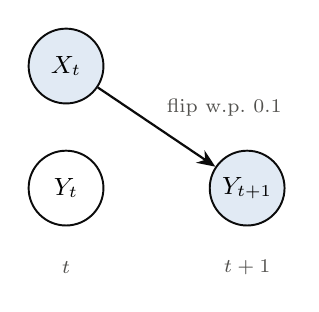
\begin{tikzpicture}[x=2.3cm, y=1.55cm]
        \node[key] (x1) at (0,0) {$X_t$};
        \node[var] (y1) at (0,-1) {$Y_t$};
        \node[key] (y2) at (1,-1) {$Y_{t+1}$};
        \draw[arr] (x1) -- node[above right, lab] {flip w.p.\ 0.1} (y2);
        \foreach \t/\l in {0/t, 1/t+1} \node[tick] at (\t,-1.65) {$\l$};
      \end{tikzpicture}
    \end{column}
  \end{columns}
\end{frame}

\subsection{Hidden driver}

\begin{frame}{System 1: a hidden driver with staggered delays}
  \begin{columns}[c]
    \begin{column}{0.47\textwidth}
      A hidden coin $Z$ is flipped every step.
      \begin{itemize}
        \item $X$ copies $Z$ after \textbf{one} step.
        \item $Y$ copies $Z$ after \textbf{two} steps.
        \item Each copy is faithful with strength $c$ (correlation $c$; $c = 1$ means a perfect copy).
      \end{itemize}
      \medskip
      There is \textbf{no arrow} from $X$ to $Y$. But $X$ sees $Z$ one step before $Y$ does,
      so $X$ \emph{predicts} $Y$'s next value.
      \medskip

      \aside{This is the ice-cream problem, stretched out in time.}
    \end{column}
    \begin{column}{0.5\textwidth}
      \centering
      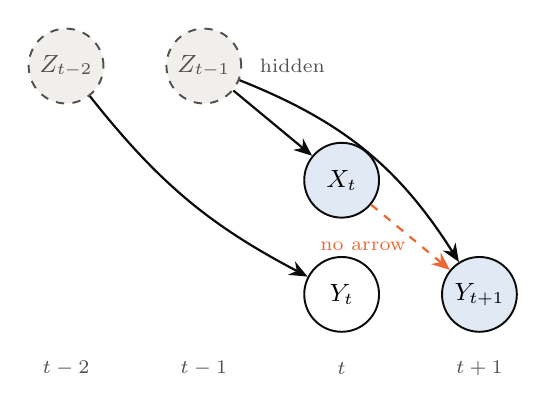
\begin{tikzpicture}[x=1.75cm, y=1.45cm]
        \node[hid] (z2) at (0,1) {$Z_{t-2}$};
        \node[hid] (z1) at (1,1) {$Z_{t-1}$};
        \node[key] (x) at (2,0) {$X_t$};
        \node[var] (y1) at (2,-1) {$Y_t$};
        \node[key] (y2) at (3,-1) {$Y_{t+1}$};
        \draw[arr] (z1) -- (x);
        \draw[arr] (z2) to[bend right=12] (y1);
        \draw[arr] (z1) to[bend left=18] (y2);
        \draw[noarrow] (x) -- node[below left=-1mm, font=\scriptsize, text=sOrange] {no arrow} (y2);
        \foreach \t/\l in {0/t-2, 1/t-1, 2/t, 3/t+1} \node[tick] at (\t,-1.65) {$\l$};
        \node[lab, right=1mm of z1] {hidden};
      \end{tikzpicture}
    \end{column}
  \end{columns}
\end{frame}

\begin{frame}{Hidden driver: transfer entropy sees a flow that isn't there}
  \begin{columns}[c]
    \begin{column}{0.56\textwidth}
      \centering
      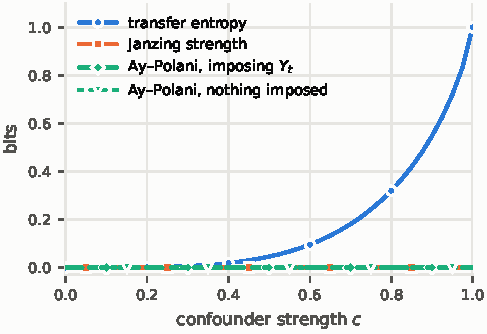
\includegraphics[width=\linewidth]{sweep_confounded_lags.pdf}
    \end{column}
    \begin{column}{0.42\textwidth}
      \begin{itemize}
        \item \textbf{Transfer entropy} rises to 1 bit as $c \to 1$:
          \[ \mathrm{TE} = 1 - h\!\left(\tfrac{1 - c^2}{2}\right) \]
          It reads $0.55$ bits at $c = 0.9$.
        \item \textbf{Both causal measures} are exactly $0$ for every $c$.
          Setting $X_t$ by hand does nothing to $\Yn$, and there is no wire to cut.
      \end{itemize}
      \medskip
      TE answers ``does $X$ help \emph{predict} $Y$?''. Here the answer is yes, even though $X$ has no causal effect on $Y$.
    \end{column}
  \end{columns}
\end{frame}

\begin{frame}{The catch: causal measures need the right graph}
  \begin{columns}[c]
    \begin{column}{0.5\textwidth}
      Suppose we can't observe $Z$. From $X$ and $Y$ alone, the natural graph to draw is the one on the right.
      \medskip

      Run both causal measures on the same data with \emph{this} graph:
      \begin{center}
        \begin{tabular}{lcc}
          \toprule & true graph & analyst's graph \\ \midrule
          TE & 0.547 & 0.547 \\
          Ay--Polani & 0 & \flagged{0.547} \\
          Janzing & 0 & \flagged{0.547} \\ \bottomrule
        \end{tabular}
      \end{center}
      \medskip
      With the wrong graph they make \textbf{exactly the same mistake as TE}.
    \end{column}
    \begin{column}{0.45\textwidth}
      \centering
      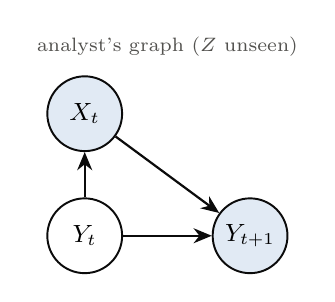
\begin{tikzpicture}[x=2.1cm, y=1.55cm]
        \node[key] (x) at (0,0) {$X_t$};
        \node[var] (y1) at (0,-1) {$Y_t$};
        \node[key] (y2) at (1,-1) {$Y_{t+1}$};
        \draw[arr] (x) -- (y2); \draw[arr] (y1) -- (y2); \draw[arr] (y1) -- (x);
        \node[lab] at (0.5,0.55) {analyst's graph ($Z$ unseen)};
      \end{tikzpicture}
      \bigskip
      \begin{block}{Lesson}
        \small The causal measures don't win because of a cleverer formula.
        They win because we \emph{handed them the truth} about the graph.
      \end{block}
    \end{column}
  \end{columns}
\end{frame}

\subsection{Synergy}

\begin{frame}{System 2: XOR, where it takes two}
  \begin{columns}[c]
    \begin{column}{0.5\textwidth}
      \[ \Yn = \Xt \oplus W \]
      with $\Xt$ and $W$ independent fair coins. Knowing only $X$ tells you \emph{nothing}
      about $Y$; knowing both tells you \emph{everything}.
      \medskip

      Two versions, which differ only in \textbf{who the partner $W$ is}:
      \begin{enumerate}
        \item $W = \Yt$: the partner is $Y$'s own past.
        \item $W = W_t$: the partner is some other signal, and $\Yt$ is irrelevant.
      \end{enumerate}
      \aside{Version 1 is the example of James, Barnett \& Crutchfield (2016).}
    \end{column}
    \begin{column}{0.46\textwidth}
      \centering
      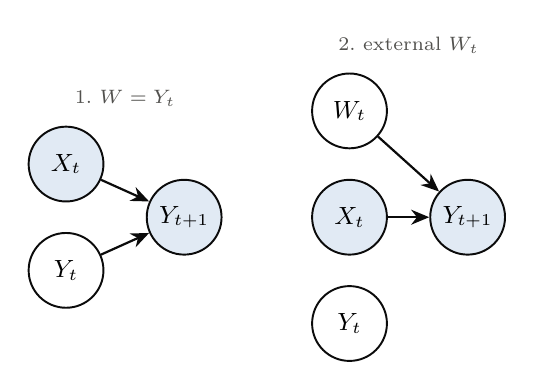
\begin{tikzpicture}[x=1.5cm, y=1.35cm]
        \node[key] (x) at (0,0) {$X_t$};
        \node[var] (y1) at (0,-1) {$Y_t$};
        \node[key] (y2) at (1,-0.5) {$Y_{t+1}$};
        \draw[arr] (x) -- (y2); \draw[arr] (y1) -- (y2);
        \node[lab] at (0.5,0.62) {1.\ $W = Y_t$};
        \begin{scope}[xshift=3.6cm]
          \node[var] (w) at (0,0.5) {$W_t$};
          \node[key] (xb) at (0,-0.5) {$X_t$};
          \node[var] (yb) at (0,-1.5) {$Y_t$};
          \node[key] (y2b) at (1,-0.5) {$Y_{t+1}$};
          \draw[arr] (w) -- (y2b); \draw[arr] (xb) -- (y2b);
          \node[lab] at (0.5,1.12) {2.\ external $W_t$};
        \end{scope}
      \end{tikzpicture}
    \end{column}
  \end{columns}
\end{frame}

\begin{frame}{XOR: the answer depends on what you condition on}
  \centering
  \renewcommand{\arraystretch}{1.3}
  \begin{tabular}{@{}lccccc@{}}
    \toprule
    & \ MI\  & \ TE\  & \ AP\  & AP $\mid \hat S$ & Janzing \\
    \midrule
    1.\ $W = \Yt$   & \flagged{0} & 1   & \flagged{0} & 1 & 1 \\
    2.\ $W = W_t$   & \flagged{0} & \flagged{0} & \flagged{0} & 1 & 1 \\
    \bottomrule
  \end{tabular}
  \par\smallskip
  {\small\color{muted} AP: flow with nothing imposed. \ $\hat S = \{\Yt\}$ in version 1 and $\{\Yt, W_t\}$ in version 2.\\
  Shaded: says ``no influence'', although $X_t$ clearly influences $\Yn$.}
  \bigskip

  \raggedright
  \begin{itemize}
    \item \textbf{Looking at $X$ alone} (MI, or flow with nothing imposed) always misses the XOR,
      because on average $X$ has no effect on $Y$.
    \item \textbf{Transfer entropy} gets 1 bit only if the partner \emph{happens to be} $Y$'s past.
      With an external partner it sees nothing.
    \item \textbf{Imposing the partner}, or \textbf{cutting the wire}, reveals the full bit either way.
  \end{itemize}
  \aside{Adding noise $\varepsilon$ to the XOR turns every 1 above into $1 - h(\varepsilon)$ and leaves the zeros at 0.}
\end{frame}

\subsection{Synchronization}

\begin{frame}{System 3: a slow signal, copied}
  \begin{columns}[c]
    \begin{column}{0.5\textwidth}
      \begin{itemize}
        \item $X$ switches slowly: it keeps its value with probability $p$, its \emph{persistence}.
        \item $Y$ copies $X$ \textbf{perfectly}, one step later: $\Yn = \Xt$.
      \end{itemize}
      \medskip
      This is the opening puzzle. $Y$ is completely driven by $X$, so the causal influence is a full bit.
      \medskip

      But when $X$ rarely changes, $Y$'s own past $\Yt = X_{t-1}$ is already a great predictor of $\Xt$,
      and so of $\Yn$.
    \end{column}
    \begin{column}{0.46\textwidth}
      \centering
      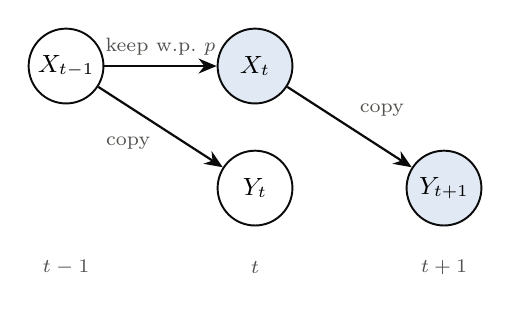
\begin{tikzpicture}[x=2.4cm, y=1.55cm]
        \node[var] (x0) at (0,0) {$X_{t-1}$};
        \node[key] (x1) at (1,0) {$X_t$};
        \node[var] (y1) at (1,-1) {$Y_t$};
        \node[key] (y2) at (2,-1) {$Y_{t+1}$};
        \draw[arr] (x0) -- node[above, lab] {keep w.p.\ $p$} (x1);
        \draw[arr] (x0) -- node[below left, lab] {copy} (y1);
        \draw[arr] (x1) -- node[above right, lab] {copy} (y2);
        \foreach \t/\l in {0/t-1, 1/t, 2/t+1} \node[tick] at (\t,-1.65) {$\l$};
      \end{tikzpicture}
    \end{column}
  \end{columns}
\end{frame}

\begin{frame}{Synchronization: perfect coupling, vanishing transfer entropy}
  \begin{columns}[c]
    \begin{column}{0.56\textwidth}
      \centering
      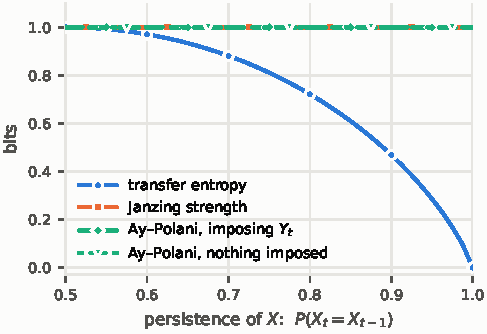
\includegraphics[width=\linewidth]{sweep_synchronized_copy.pdf}
    \end{column}
    \begin{column}{0.42\textwidth}
      \begin{itemize}
        \item \textbf{Causal measures}: 1 bit, whatever $p$ is. Setting $X_t$ fully determines $\Yn$.
        \item \textbf{Transfer entropy} $= h(p) \to 0$ as $X$ becomes predictable.
          At $p = 0.95$ it is $0.29$ bits.
      \end{itemize}
      \medskip
      TE only counts information about $\Yn$ that is \emph{new} relative to $Y$'s past.
      A perfectly coupled but predictable pair looks like almost no transfer.
      \medskip

      \aside{At $p = 1$ this is the ``synchronized chains'' example of Ay \& Polani: TE $= 0$, influence $= 1$ bit.}
    \end{column}
  \end{columns}
\end{frame}

\begin{frame}{All systems at a glance}
  \centering\small
  \renewcommand{\arraystretch}{1.25}
  \begin{tabular}{@{}lccccccc@{}}
    \toprule
    system & $X_t \to Y_{t+1}$? & MI & TE & AP & AP $\mid \hat S$ & Janzing \\
    \midrule
    Noisy wire (control)                 & yes & 0.53 & 0.53 & 0.53 & 0.53 & 0.53 \\
    Hidden driver, $c = 0.9$             & no  & \flagged{0.55} & \flagged{0.55} & 0 & 0 & 0 \\
    \quad same data, analyst's graph     & no  & \flagged{0.55} & \flagged{0.55} & \flagged{0.55} & \flagged{0.55} & \flagged{0.55} \\
    XOR, $W = Y_t$                       & yes & \flagged{0} & 1$^\dagger$ & \flagged{0} & 1 & 1 \\
    XOR, external $W_t$                  & yes & \flagged{0} & \flagged{0} & \flagged{0} & 1 & 1 \\
    Slow copy, $p = 0.95$                & yes & 1 & \flagged{0.29} & 1 & 1 & 1 \\
    \bottomrule
  \end{tabular}
  \par\medskip
  {\color{muted} Shaded: misleading about whether, or how strongly, $X_t$ influences $Y_{t+1}$.\\
  $^\dagger$ The right number for a subtle reason, as the next section shows.}
  \bigskip

  \raggedright
  Transfer entropy gives a \textbf{false positive} (hidden driver), a \textbf{false negative} (external XOR)
  and a large \textbf{underestimate} (slow copy).
\end{frame}

% ====================================================================
\section{Why they disagree}

\begin{frame}{Splitting information into kinds}
  Two sources, $\Xt$ and a partner $W$, carry information about a target $\Yn$.
  \emph{Partial information decomposition} (Williams \& Beer, 2010) splits it into four parts:
  \medskip
  \begin{columns}[c]
    \begin{column}{0.5\textwidth}
      \begin{itemize}
        \item \textbf{Redundant}: either source alone would tell you.
        \item \textbf{Unique to $X$}: only $X$ tells you.
        \item \textbf{Unique to $W$}: only $W$ tells you.
        \item \textbf{Synergistic}: only the two \emph{together} tell you, as in XOR.
      \end{itemize}
    \end{column}
    \begin{column}{0.46\textwidth}
      \centering
      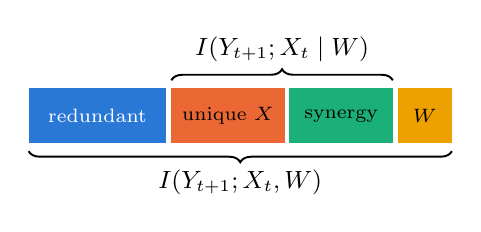
\begin{tikzpicture}[x=1.25cm]
        \fill[sBlue] (0,0) rectangle (1.4,0.7);
        \fill[sOrange] (1.45,0) rectangle (2.6,0.7);
        \fill[sAqua] (2.65,0) rectangle (3.7,0.7);
        \fill[sYellow] (3.75,0) rectangle (4.3,0.7);
        \node[font=\scriptsize, text=white] at (0.7,0.35) {redundant};
        \node[font=\scriptsize] at (2.025,0.35) {unique $X$};
        \node[font=\scriptsize] at (3.175,0.35) {synergy};
        \node[font=\scriptsize] at (4.025,0.35) {$W$};
        \draw[decorate, decoration={brace, amplitude=4pt}, line width=0.7pt] (1.45,0.8) -- (3.7,0.8)
          node[midway, above=3pt, font=\small] {$I(\Yn;\Xt \mid W)$};
        \draw[decorate, decoration={brace, amplitude=4pt, mirror}, line width=0.7pt] (0,-0.1) -- (4.3,-0.1)
          node[midway, below=3pt, font=\small] {$I(\Yn;\Xt, W)$};
      \end{tikzpicture}
    \end{column}
  \end{columns}
  \bigskip
  \begin{block}{The identity that explains transfer entropy}
    With the partner $W = \Yt$:\qquad
    $\mathrm{TE} = I(\Yn;\Xt \mid \Yt) = \text{unique to } X + \text{synergy}$
    \smallskip

    TE leaves out the redundant part, and counts synergy as if it belonged to $X$ alone.
  \end{block}
\end{frame}

\begin{frame}{What transfer entropy is made of}
  \centering
  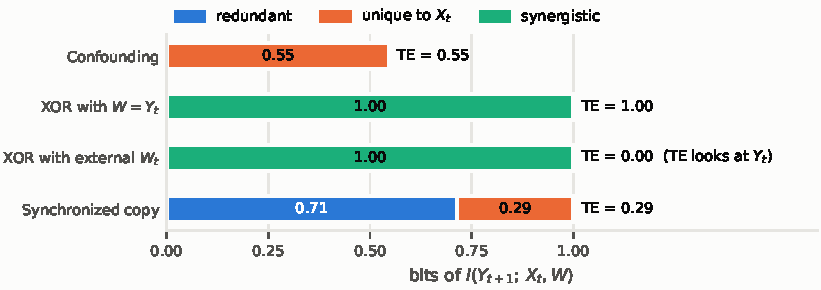
\includegraphics[width=0.84\linewidth]{pid_by_system.pdf}
  \par\smallskip
  \raggedright\small
  \begin{columns}[T]
    \begin{column}{0.48\textwidth}
      \begin{itemize}
        \item \textbf{XOR, $W = Y_t$}: the whole bit is \emph{synergy}. TE credits it to $X$,
          although it exists only in the pair.
        \item \textbf{External XOR}: synergy between $X_t$ and $W_t$. TE's partner is $Y_t$,
          so it sees none of it.
      \end{itemize}
    \end{column}
    \begin{column}{0.48\textwidth}
      \begin{itemize}
        \item \textbf{Slow copy}: most of the bit is \emph{redundant} with $Y$'s past, and TE drops it.
        \item \textbf{Hidden driver}: looks like clean \emph{unique} information. The decomposition
          is observational too, so it can't see $Z$.
      \end{itemize}
    \end{column}
  \end{columns}
\end{frame}

\begin{frame}{Slow copy: redundancy crowds out transfer entropy}
  \begin{columns}[c]
    \begin{column}{0.5\textwidth}
      \centering
      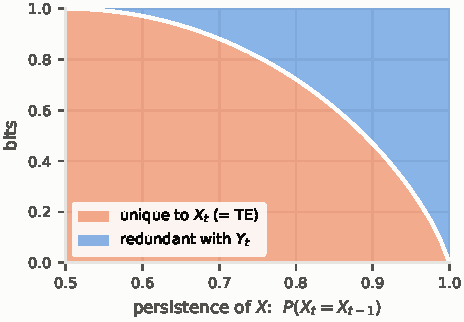
\includegraphics[width=\linewidth]{pid_copy_sweep.pdf}
    \end{column}
    \begin{column}{0.46\textwidth}
      Together $\Xt$ and $\Yt$ always know the full 1 bit about $\Yn$.
      \medskip

      As $X$ becomes more persistent, more of that bit is also known to $Y$'s past,
      because $\Yt = X_{t-1}$ usually equals $\Xt$. That part is redundant.
      \medskip

      TE keeps only the \textbf{unique} part, $h(p)$. It measures \emph{new} information, not coupling strength.
    \end{column}
  \end{columns}
\end{frame}

% ====================================================================
\section{Real data, and takeaways}

\begin{frame}{With finite data it gets worse}
  \begin{columns}[c]
    \begin{column}{0.54\textwidth}
      \centering
      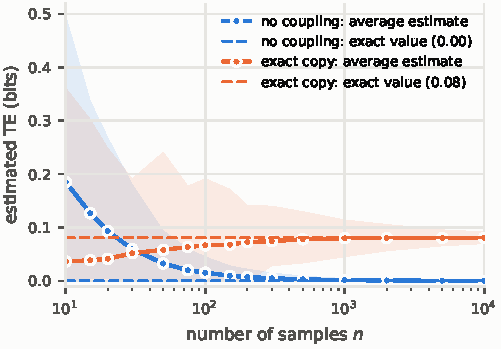
\includegraphics[width=\linewidth]{finite_sample.pdf}\\
      \aside{Shaded: middle 90\% of 2,000 repeated experiments.}
    \end{column}
    \begin{column}{0.44\textwidth}
      In practice we \emph{estimate} TE: count how often each outcome occurs in $n$ samples,
      then plug the frequencies into the formula.
      \begin{itemize}
        \item With \textbf{no coupling at all}, the average estimate is $0.19$ bits at $n = 10$
          and $0.015$ at $n = 100$. It shrinks only like $1/(n \ln 2)$.
        \item For a deterministic copy the estimate is biased \emph{downward}.
        \item For $n \le 30$ the uncoupled system looks \emph{more} ``causal'' than the perfectly coupled one.
      \end{itemize}
      \aside{Always compare an estimate against a null, such as shuffled data.}
    \end{column}
  \end{columns}
\end{frame}

\begin{frame}{Takeaways}
  \begin{enumerate}
    \setlength{\itemsep}{2.5mm}
    \item \textbf{Transfer entropy measures prediction, not causation.} It answers
      ``does $X$ help forecast $Y$ beyond $Y$'s past?''. That question has a different answer from
      ``does $X$ influence $Y$?'' when there is
      \begin{itemize}
        \item a hidden common driver (false positive),
        \item synergy with another input (misattributed, or missed entirely),
        \item a predictable, synchronized source (underestimate).
      \end{itemize}
    \item \textbf{Interventional measures fix this, given the right causal graph.}
      With the wrong graph they inherit the same errors.
    \item \textbf{Finite samples add spurious transfer entropy} of about $1/(n \ln 2)$ bits, so test against a null.
    \item \textbf{Pick the measure that matches your question}: forecasting, or ``what if I intervened?''.
  \end{enumerate}
\end{frame}

\begin{frame}{Questions to think about}
  \begin{enumerate}
    \setlength{\itemsep}{3mm}
    \item In the hidden-driver system, which extra variable would you condition on to make
      transfer entropy report 0? What does that suggest about using TE in practice?
    \item In the slow-copy system, TE $\to 0$ as $X$ becomes predictable.
      Is that a bug or a feature? When would you \emph{want} this behavior?
    \item For the XOR, Ay--Polani flow is 0 with nothing imposed and 1 bit when imposing $W$.
      Which one is ``the'' causal influence of $X$? Do we need to choose?
    \item Why is the plug-in estimate biased \emph{upward} with no coupling, but \emph{downward}
      for a deterministic copy? \aside{Hint: think about outcomes that never show up in a small sample.}
  \end{enumerate}
\end{frame}

\begin{frame}{References and code}
  \small
  \begin{itemize}
    \setlength{\itemsep}{1.5mm}
    \item T.\ Schreiber (2000). Measuring information transfer. \emph{Phys.\ Rev.\ Lett.} 85, 461.
    \item N.\ Ay \& D.\ Polani (2008). Information flows in causal networks. \emph{Adv.\ Complex Syst.} 11, 17.
    \item D.\ Janzing, D.\ Balduzzi, M.\ Grosse-Wentrup \& B.\ Sch\"olkopf (2013).
      Quantifying causal influences. \emph{Ann.\ Stat.} 41, 2324.
    \item R.\ G.\ James, N.\ Barnett \& J.\ P.\ Crutchfield (2016).
      Information flows? A critique of transfer entropies. \emph{Phys.\ Rev.\ Lett.} 116, 238701.
    \item P.\ L.\ Williams \& R.\ D.\ Beer (2010). Nonnegative decomposition of multivariate information. arXiv:1004.2515.
    \item J.\ Pearl (2009). \emph{Causality}, 2nd ed. Cambridge University Press. \aside{(seeing vs.\ doing)}
  \end{itemize}
  \bigskip
  \textbf{Code:} every number in these slides is computed exactly in the \texttt{causality-measures}
  repository (Python, \texttt{dit}). Run \texttt{uv run pytest}, then the scripts in \texttt{experiments/}.
\end{frame}

\end{document}
